\documentclass[10pt,twocolumn]{article}

\usepackage[margin=1in]{geometry}
\usepackage{graphicx}
\usepackage{booktabs}
\usepackage{array}
\usepackage{amsmath}
\usepackage{hyperref}
\usepackage{microtype}
\usepackage{xcolor}
\usepackage{float}
\usepackage{enumitem}

\graphicspath{{figures/}{../results/plots/}}

\newcommand{\TODO}[1]{\textcolor{red}{[TODO: #1]}}

\title{\textbf{Gipfelsturm: Efficient Training Recipes\\for a 125M--3B Language Model}\\[0.5em]
\large ETH Zurich --- Large Scale AI Engineering, Spring 2026}

\author{
  Zhiyao Yan \and
  Xin Wei \and
  Yuyan Wang Ying
}

\date{}

\begin{document}

\maketitle

% ─────────────────────────────────────────────────────────────────────────────
\begin{abstract}
We address Gipfelsturm Challenge~1: achieving the lowest validation loss on
Nemotron-ClimbMix within a strict 30-minute wall-clock window on the Clariden
supercomputer (NVIDIA GH200). Rather than fixing a token budget, we treat
wall-clock time as the only constraint and systematically optimise three
levers (model size, batch size, and learning rate schedule) using short
proxy experiments to inform the final run. We find that WSD with 20\% decay on 760M (4 nodes, GBS=256) achieves the best trade-off between
per-GPU throughput and convergence speed, yielding a final validation loss of
2.369.
\end{abstract}

% ─────────────────────────────────────────────────────────────────────────────
\section{Motivation}

Training large language models efficiently under strict compute budgets is
central to modern deep learning practice. Standard scaling laws
\cite{chinchilla} characterise optimal token allocation for a \emph{fixed}
compute budget; however, our setting imposes a \emph{fixed wall-clock time}
of 30 minutes instead. This shifts the optimisation target: we must jointly
maximise system throughput (tokens processed per second) \emph{and}
algorithmic convergence (loss reduction per token), since both affect the
final validation loss.

The Clariden cluster provides up to 4 nodes of 4$\times$ GH200 GPUs each
(16 GPUs, 16 GPU-hours in 30 minutes). Within this budget the natural model
scale is 125M--3B parameters. Our goal is to find,
through systematic experimentation, the configuration that minimises
validation loss before the clock runs out.

% ─────────────────────────────────────────────────────────────────────────────
\section{Setup}

\paragraph{Infrastructure.}
Experiments run on Clariden (CSCS) using nodes with 4$\times$ NVIDIA GH200
GPUs (96\,GB HBM3 each). The GH200 integrates a Grace CPU and Hopper GPU
via NVLink-C2C (900\,GB/s), and nodes connect over Slingshot-11.

\paragraph{Framework.}
We use Megatron-LM (core v0.16.1)~\cite{megatron} with data parallelism
(TP=1, PP=1), BF16 mixed precision, TransformerEngine for fused kernels, and
a distributed optimizer with overlapped gradient reduction.

\paragraph{Dataset \& Tokenizer.}
Training uses Nemotron-ClimbMix~\cite{climbmix}, a curated pre-training
corpus stored in Megatron binary format. The GPT-2 BPE tokeniser (50,257
vocab, sequence length 4,096) enables direct comparison with nanoGPT
baselines~\cite{nanogpt}.

\paragraph{Model Architecture.}
All models are decoder-only transformers with RoPE embeddings, RMSNorm,
SwiGLU, grouped-query attention (GQA), and untied embeddings.
Table~\ref{tab:model-configs} lists the configurations evaluated.

\begin{table}[H]
\centering
\small
\begin{tabular}{lrrrrr}
\toprule
Size & Layers & Hidden & FFN  & Heads & KV \\
\midrule
125M & 12 & 768  & 2048  & 12 & 4 \\
350M & 24 & 1024 & 2816  & 16 & 4 \\
760M & 24 & 1536 & 4096  & 16 & 4 \\
1.5B & 48 & 1600 & 4352  & 20 & 4 \\
3B   & 32 & 3072 & 8192  & 24 & 8 \\
\bottomrule
\end{tabular}
\caption{Model configurations evaluated.}
\label{tab:model-configs}
\end{table}

% ─────────────────────────────────────────────────────────────────────────────
\section{Method}

Our pipeline has three sequential stages.

\subsection{Stage 1: Throughput Benchmarking}

We run 50-step jobs for each model size and batch size to measure empirical
throughput (tokens/sec/GPU), averaging over steps 10--50 to exclude JIT
compilation overhead. This gives the number of training steps that fit within
30 minutes:
\[
  N_{\text{steps}} = \frac{\text{tok/s/GPU} \times N_{\text{GPU}} \times
  1800\,\text{s}}{\text{GBS} \times L_{\text{seq}}}
\]
We sweep model sizes (125M--3B), global batch sizes GBS $\in \{128,256,512\}$,
and node counts $\in \{1,2,4\}$ for the best candidate models.

\subsection{Stage 2: Proxy Ablations (500 steps, 1 node)}

Using the model selected from Stage~1, we run two ablation groups.

\paragraph{Learning rate schedule.}
We compare cosine annealing against Warmup-Stable-Decay
(WSD)~\cite{minicpm} with decay fractions of 20\%, 30\%, and 40\% of total
steps. WSD decouples the stable training phase from the final decay, which
may exploit the wall-clock budget more effectively. All runs use
$\text{lr}=3\!\times\!10^{-4}$, $\text{min-lr}=3\!\times\!10^{-5}$, 100
warmup steps.

\paragraph{Batch size trade-off.}
We compare GBS $\in \{128, 256\}$ with cosine LR at 500 steps. Larger
batches improve hardware utilisation but yield fewer gradient updates in a
fixed time budget. GBS=512 was eliminated after Stage~1 showed it yields
only 157 steps in 30 minutes on a single node.

\subsection{Stage 3: Final 30-Minute Run}

We submit a single job on 4 nodes with the best configuration from
Stages~1--2, running for exactly $N_{\text{steps}}$ steps as computed
from the measured throughput.

% ─────────────────────────────────────────────────────────────────────────────
\section{Evaluation}

\subsection{Throughput Benchmarking}

Table~\ref{tab:throughput} reports empirical throughput and the resulting
30-minute step budgets computed by applying the formula from Section~3.1
with the measured GBS and actual GPU count. All averages exclude the
first 10 iterations to eliminate JIT warmup noise.
Figure~\ref{fig:throughput-model} shows throughput vs.\ model size;
Figure~\ref{fig:scaling} shows multi-node scaling efficiency for the 760M
model.

\begin{table}[H]
\centering
\small
\begin{tabular}{llrrr}
\toprule
Model & Config & Tok/s/GPU & GPUs & Steps/30\,min \\
\midrule
125M & 1n, GBS256 & 57,005 & 4  & 391  \\
350M & 1n, GBS256 & 79,113 & 4  & 543  \\
760M & 1n, GBS128 & 54,276 & 4  & 745  \\
760M & 1n, GBS256 & 48,179 & 4  & 330  \\
760M & 1n, GBS512 & 45,776 & 4  & 157  \\
760M & 2n, GBS256 & 42,832 & 8  & 588  \\
760M & 4n, GBS256 & 37,828 & 16 & \textbf{1,039} \\
350M & 4n, GBS256 & 38,586 & 16 & 1,060 \\
1.5B & 1n, GBS256 & 35,005 & 4  & 240  \\
3B   & 1n, GBS256 & 20,183 & 4  & 138  \\
\bottomrule
\end{tabular}
\caption{Empirical throughput and projected 30-min step budget.
Steps are computed with the actual GPU count and GBS for each run.}
\label{tab:throughput}
\end{table}

\begin{figure}[H]
  \centering
  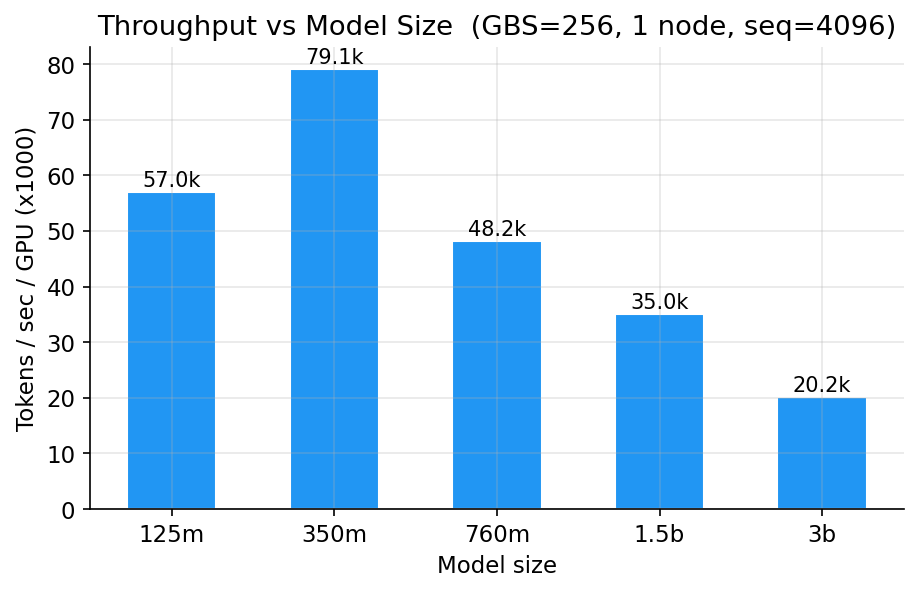
\includegraphics[width=\linewidth]{throughput_model_size.png}
  \caption{Throughput vs.\ model size (GBS=256, 1 node). The 350M model
  peaks at 79,113\,tok/s/GPU, likely due to a favourable
  compute-to-memory-bandwidth ratio at this scale.}
  \label{fig:throughput-model}
\end{figure}

\begin{figure}[H]
  \centering
  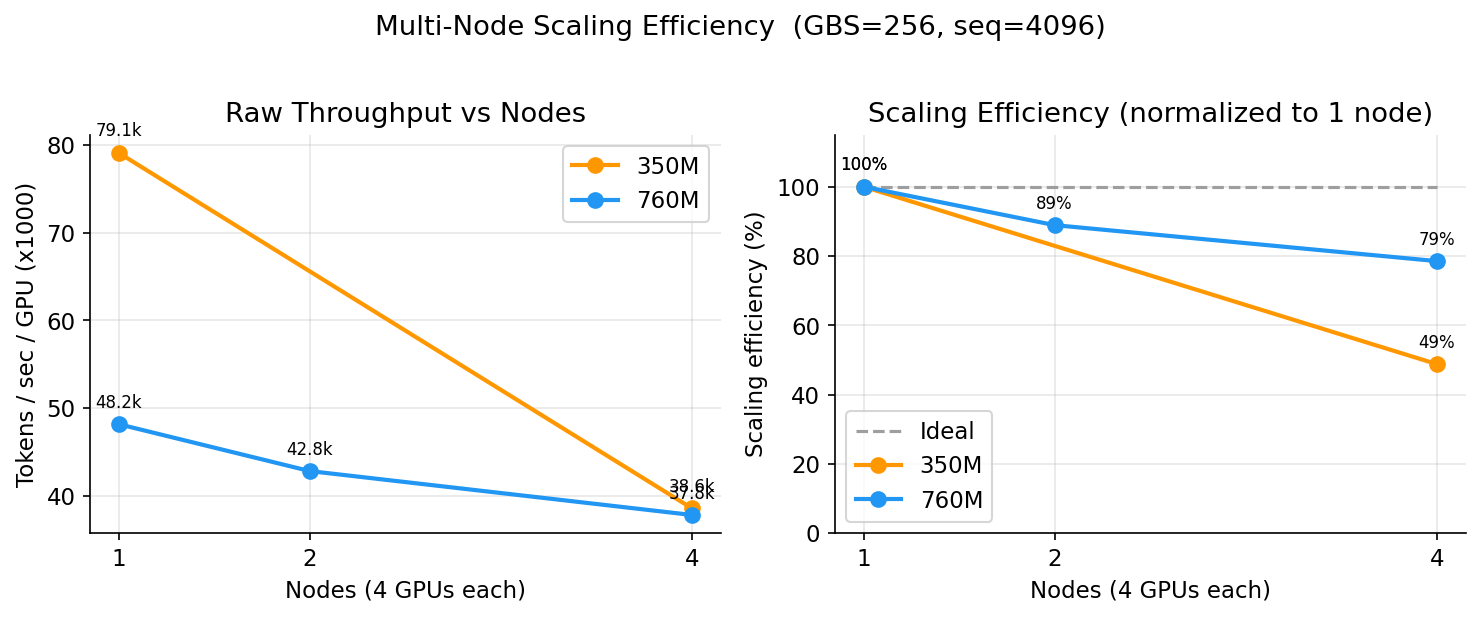
\includegraphics[width=\linewidth]{scaling_efficiency.png}
  \caption{Multi-node scaling efficiency for 760M and 350M (GBS=256). At 4
  nodes, 760M retains 78.5\% of single-node throughput (37,828 vs.\
  48,179\,tok/s/GPU) while 350M drops to 48.8\% (38,586 vs.\
  79,113\,tok/s/GPU). Despite its single-node advantage, 350M is not
  competitive at 4 nodes.}
  \label{fig:scaling}
\end{figure}

\paragraph{Model selection.}
Despite 350M having higher single-node throughput (79,113 vs.\
48,179\,tok/s/GPU), its poor multi-node scaling (48.8\%) makes it
roughly equivalent to 760M at 4 nodes in projected step count (1,060
vs.\ 1,039 steps). Since 760M has 2$\times$ the parameter count we
select \textbf{760M on 4 nodes, GBS=256} for all ablations and the
final run, projecting 1,039 gradient steps and approximately
\textbf{1.09 billion tokens} processed in 30 minutes
($1039 \times 256 \times 4096 \approx 1.09\,\text{B}$).

\subsection{Batch Size Hardware Trade-off}

\begin{figure}[!tbp]
  \centering
  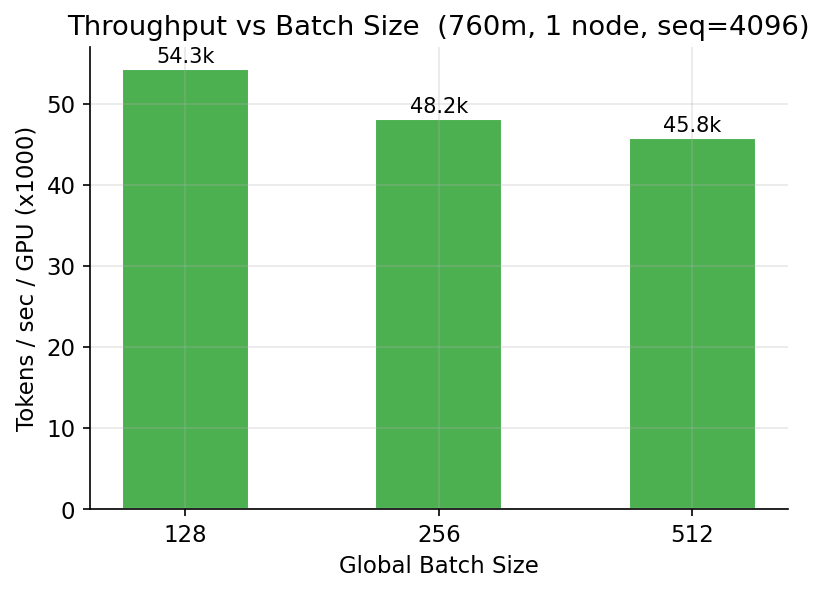
\includegraphics[width=\linewidth]{throughput_batch_size.png}
  \caption{Throughput vs.\ global batch size for the 760M model (1 node).
  Larger batches increase GPU utilisation but yield fewer gradient updates
  in a fixed time. GBS=512 is eliminated: 157 steps/30\,min is too few for
  meaningful convergence.}
  \label{fig:batchsize-thr}
\end{figure}

Figure~\ref{fig:batchsize-thr} shows the throughput trade-off across
GBS=128, 256, and 512 for the 760M model. GBS=128 achieves the highest
throughput (54,276\,tok/s/GPU) but yields fewer tokens per step, while
GBS=256 balances utilisation and gradient signal. GBS=512 is eliminated on
throughput grounds alone. The convergence comparison between GBS=128
and GBS=256 is shown in Figure~\ref{fig:batchsize-conv}.

\begin{figure}[!tbp]
  \centering
  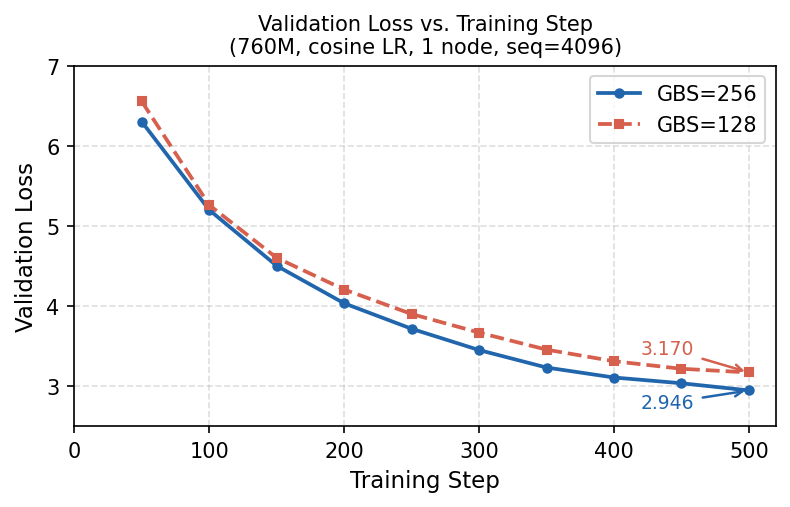
\includegraphics[width=\linewidth]{batchsize_val_loss.png}
  \caption{Validation loss curves for GBS=128 vs.\ GBS=256 (760M, 500
  steps, cosine LR, 1 node). GBS=256 converges to a lower final validation loss (2.946 vs. 3.170), a gap of 0.224 nats, despite its lower per-GPU throughput.}
  \label{fig:batchsize-conv}
\end{figure}



\begin{table}[H]
\centering
\small
\caption{Batch size ablation results (760M, cosine LR, 500 steps, 1 node, full validation set).}
\label{tab:batchsize-results}
\begin{tabular}{lrrr}
\toprule
GBS & Tok/s/GPU & Train Loss & Val Loss \\
\midrule
128 & 54,276 & 3.190 & 3.158 \\
256 & 48,179 & 2.935 & 2.960 \\
\bottomrule
\end{tabular}
\end{table}

GBS=256 achieves a final validation loss of 2.946, outperforming GBS=128 (3.170) by 0.224 nats despite its lower raw throughput. The gap widens steadily across all 500 steps, indicating that GBS=128 is gradient-update-limited: although it processes more tokens per second, the fewer gradient updates yield weaker convergence. We therefore select GBS=256 for all ablation and final runs.


\subsection{Learning Rate Schedule Ablation}

\begin{figure}[!tbp]
  \centering
  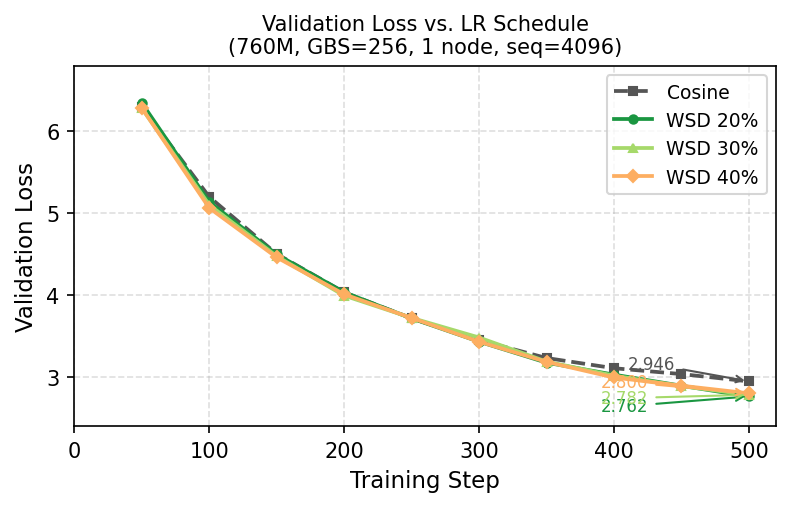
\includegraphics[width=\linewidth]{lr_val_loss.png}
  \caption{Validation loss for cosine vs.\ WSD schedules (760M, GBS=256,
  500 steps, 1 node). All WSD variants outperform cosine, with WSD 20\% achieving the lowest final validation loss of 2.762.}
  \label{fig:lr-val}
\end{figure}

\begin{table}[!tbp]
\centering
\small
\caption{LR schedule ablation results (760M, GBS=256, 500 steps, 1 node).}
\label{tab:lr-results}
\begin{tabular}{lrr}
\toprule
Schedule    & Train Loss & Val Loss \\
\midrule
Cosine      & 2.935 & 2.946 \\
WSD 20\%    & 2.784 & 2.762 \\
WSD 30\%    & 2.797 & 2.782 \\
WSD 40\%    & 2.812 & 2.800 \\
\bottomrule
\end{tabular}
\end{table}

Figure~\ref{fig:lr-val} reveals a clear advantage for WSD over cosine annealing across all decay fractions. The four schedules track nearly identically for the first 300 steps; divergence emerges in the decay phase (steps 400–500), where WSD's sharp final drop drives rapid convergence. WSD 20\% achieves the best final validation loss of 2.762, a margin of 0.184 nats over cosine (2.946). Among WSD variants, shorter decay fractions perform better within this 500-step budget: WSD 20\% $>$ WSD 30\% $>$ WSD 40\%, suggesting that a longer stable phase is more valuable than a longer decay when the total step count is small. We select WSD with 20\% decay for the final run.


\subsection{Final 30-Minute Run}

\begin{figure}[H]
  \centering
  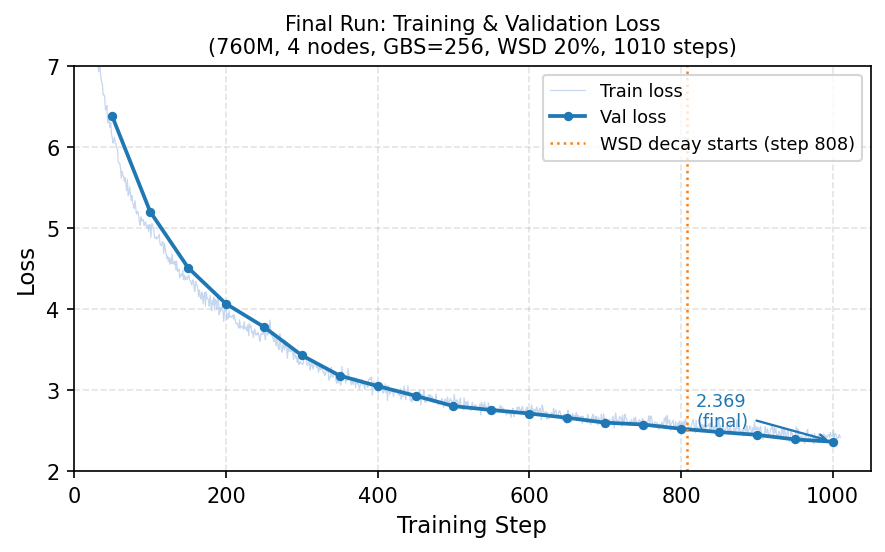
\includegraphics[width=\linewidth]{figures/final_760m_WSD20.png}
  \caption{Training and validation loss for the final 30-minute run
  (760M, 4 nodes, GBS=256, schedule=WSD20, 1010 training steps).}
  \label{fig:final}
\end{figure}

Our final configuration achieves a validation loss of 2.369
after 1000 training steps, processing approximately 1.05B tokens
in 30 minutes.

% ─────────────────────────────────────────────────────────────────────────────
\section{Conclusion}

We showed that systematic throughput benchmarking and short proxy ablations
are sufficient to identify near-optimal configurations under a strict
wall-clock budget. Key findings: (1)~per-GPU throughput does not translate
directly to multi-node step count---350M's 64\% single-node throughput
advantage over 760M completely vanishes at 4 nodes due to its 48.8\%
scaling efficiency vs.\ 78.5\% for 760M;
(2)~WSD consistently outperforms cosine annealing, with WSD 20\% achieving the best validation loss (2.762 vs. 2.946 for cosine, a margin of 0.184 nats); within WSD variants, shorter decay fractions are preferable under a short step budget;
(3)~GBS=256 outperforms GBS=128 in final validation loss (2.946 vs. 3.158) despite lower per-GPU throughput, as larger batches provide stronger gradient signal per update.
Our final model achieves a validation loss of 2.369 in 30 minutes.

% ─────────────────────────────────────────────────────────────────────────────
\bibliographystyle{plain}
\begin{thebibliography}{9}

\bibitem{chinchilla}
J.~Hoffmann et al.
\textit{Training Compute-Optimal Large Language Models (Chinchilla)}, 2022.

\bibitem{minicpm}
S.~Hu et al.
\textit{MiniCPM: Unleashing the Potential of Small Language Models with WSD
LR Scheduler}, 2024.

\bibitem{nanogpt}
A.~Karpathy.
\textit{nanoGPT}, GitHub, 2022.

\bibitem{megatron}
M.~Shoeybi et al.
\textit{Megatron-LM: Training Multi-Billion Parameter Language Models Using
Model Parallelism}, arXiv:1909.08053, 2019.

\bibitem{climbmix}
NVIDIA.
\textit{Nemotron-ClimbMix: A Curated Pre-training Corpus}, 2025.

\end{thebibliography}

\end{document}
